\documentclass[letterpaper]{article}

\usepackage{fancyvrb}
\usepackage{fullpage}
\usepackage{listings}
\usepackage{xcolor}
\usepackage{float}
\usepackage{hyperref}

\lstset{basicstyle=\ttfamily, 
        backgroundcolor=\color[gray]{0.95}}
        
\author{Michael Gruenstaeudl, Nils Jenke}
\title{Using PACViR}

\usepackage{Sweave}
\begin{document}
\Sconcordance{concordance:PACViR_Vignette.tex:PACViR_Vignette.Rnw:%
1 15 1 1 0 3 1 1 4 16 1 5 0 1 4 9 1 1 3 2 0 1 3 1 0 1 %
1 1 2 6 1 4 0 1 3 35 1 1 2 24 0 1 2 1 1}

%\SweaveUTF8


\maketitle

\tableofcontents

\section{Introduction}

  \textbf{PACViR} is a user-friendly software tool to visualize the coverage depth of a complete plastid genome as well as the equality of its IR regions while simultaneously accounting for the circular, quadripartite structure of the genome. This vignette provides two examples of executing PACViR on empirical data via the R function '\textit{PACViR.complete()}' from within the R interpreter and from the BASH commandline shell.

\section{Requirements}

  To run PACViR, several dependencies have to be installed.


  \begin{footnotesize}
  \begin{lstlisting}[linerange=\\begin\{Sinput\}-\\end\{Sinput\},includerangemarker=false]
\begin{Schunk}
\begin{Sinput}
>     #TO DO: List dependencies and their installation here.
>     #library(PACViR)
\end{Sinput}
\end{Schunk}
  \end{lstlisting}
  \end{footnotesize}

\pagebreak

\section{Executing PACViR via R interpreter}
PACViR can be executed via the R function '\textit{PACViR.complete()}' from within the R interpreter.

\begin{footnotesize}
\begin{lstlisting}[linerange=\\begin\{Sinput\}-\\end\{Sinput\},includerangemarker=false]
\begin{Schunk}
\begin{Sinput}
# MH161174
## Specify input files
gbkFile <- system.file("extdata", "MH161174/MH161174.gb", package="PACViR")
bamFile <- system.file("extdata", "MH161174/MH161174_PlastomeReadsOnly.sorted.bam", 
                       package="PACViR")
## Specify output file
outFile <- paste(getwd(), "/MH161174_AssemblyCoverage_viz.svg", sep="")
## Run PACViR
PACViR.complete(gbk.file=gbkFile, bam.file=bamFile, windowSize=250, 
                mosdepthCmd='mosdepth', threshold=15, delete=FALSE, 
                output=outFile)
\end{Sinput}
\end{Schunk}
\end{lstlisting}
\end{footnotesize}
  
\begin{figure}[H]
\centering
    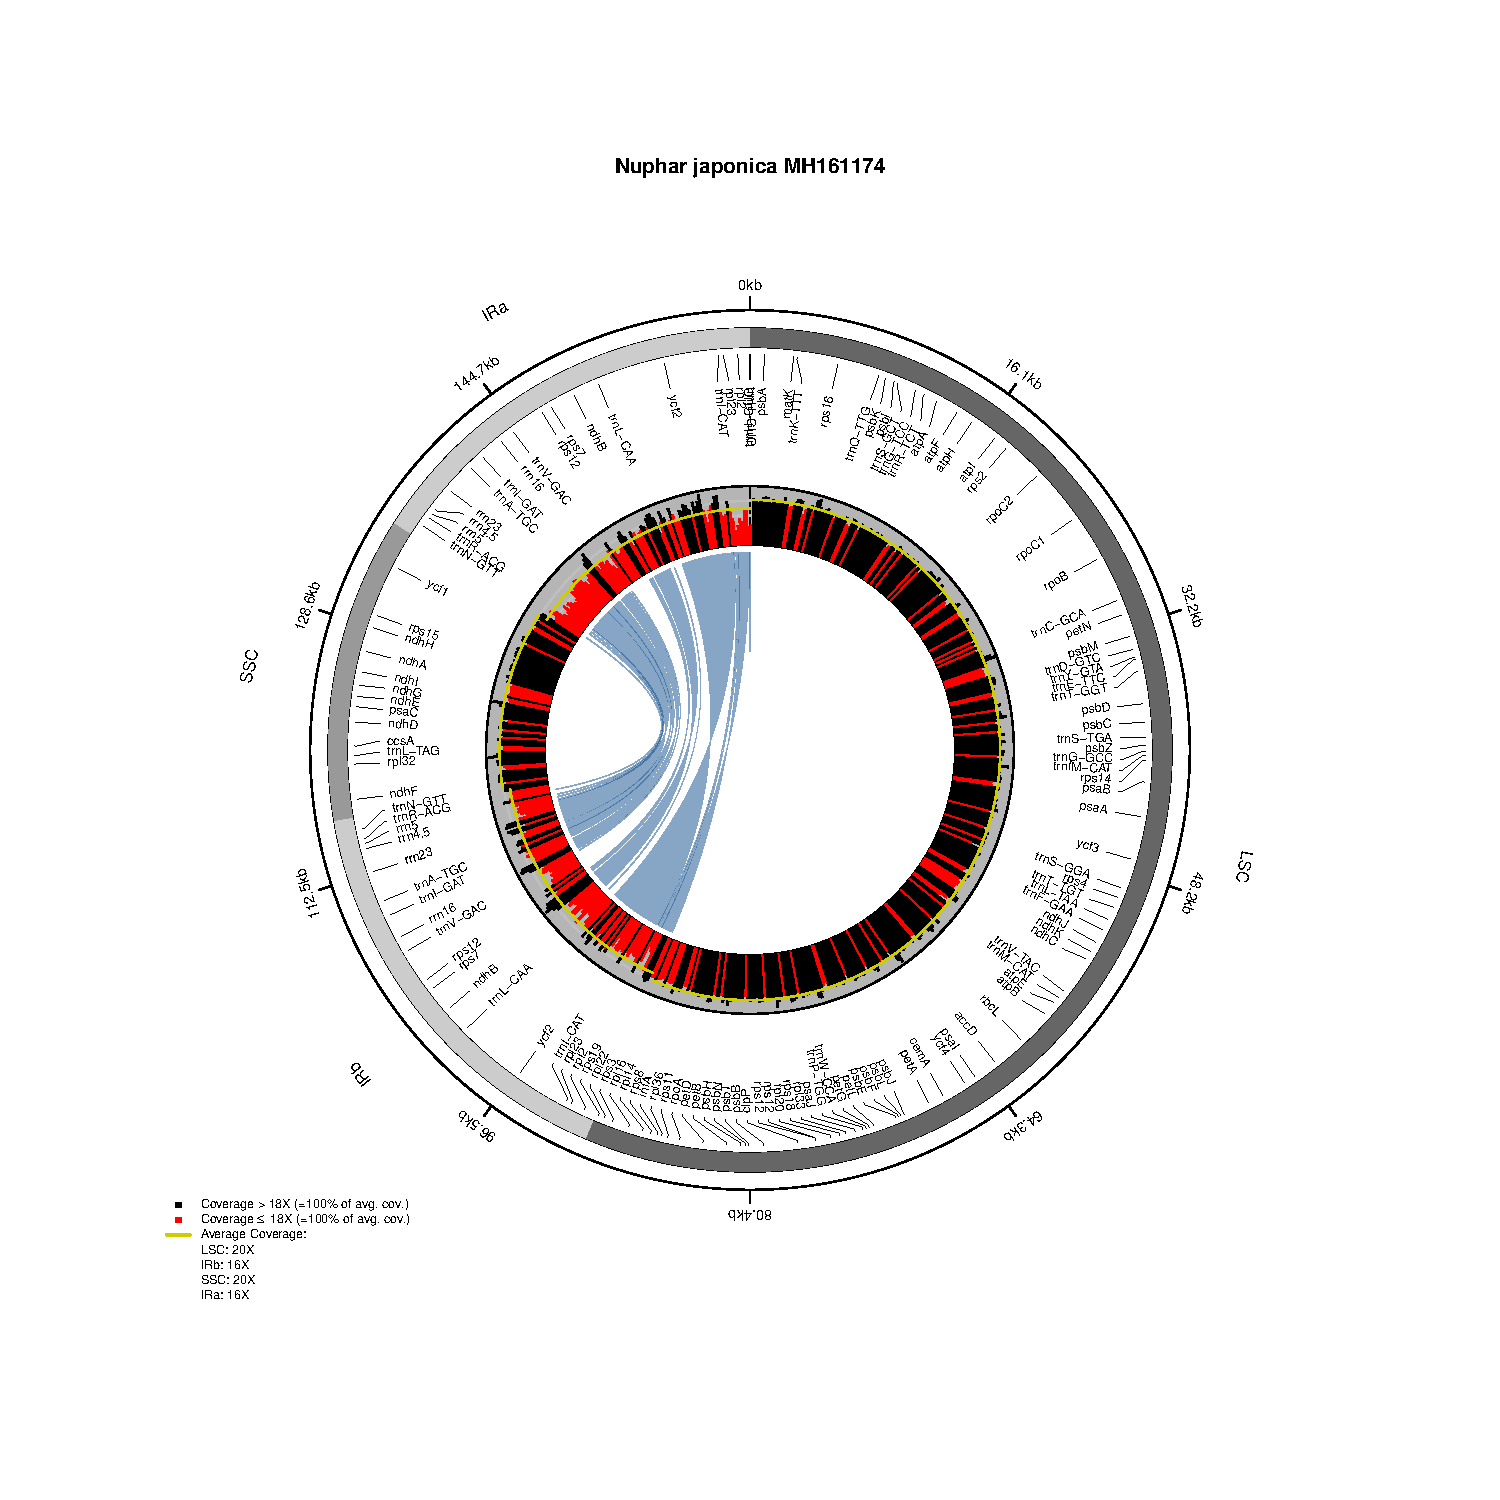
\includegraphics{MH161174_AssemblyCoverage_viz.pdf}
    \caption{File '\textit{MH161174\_AssemblyCoverage\_viz.svg}' as generated via '\textit{PACViR.complete()}'}
\centering
\end{figure}

\pagebreak

\section{Executing PACViR via BASH shell}
PACViR can be executed via the BASH shell command '\textit{PACViR\_Rscript.R}' from the BASH commandline shell.
  
\begin{footnotesize}
\begin{lstlisting}
# MH899017
Rscript ./inst/extdata/PACViR_Rscript.R  \
     -k ./inst/extdata/MH899017.gb \
     -b ./inst/extdata/MH899017_PlastomeReadsOnly.sorted.bam \
     -o ./MH899017_AssemblyCoverage_viz.svg
\end{lstlisting}
\end{footnotesize}

\begin{figure}[H]
\centering
    \includegraphics{MH899017_AssemblyCoverage_viz.pdf}
    \caption{File '\textit{MH899017\_AssemblyCoverage\_viz.svg}' as generated via '\textit{PACViR\_Rscript.R}'}
\centering
\end{figure}

\pagebreak

%\section{Modifying parameters}

%  Depending on which system PACViR will be executed

%\section{More Information}

\section{sessionInfo}

\begin{Schunk}
\begin{Sinput}
> sessionInfo()
\end{Sinput}
\begin{Soutput}
R version 3.3.3 (2017-03-06)
Platform: x86_64-pc-linux-gnu (64-bit)
Running under: Debian GNU/Linux 9 (stretch)

locale:
 [1] LC_CTYPE=de_DE.UTF-8       LC_NUMERIC=C              
 [3] LC_TIME=de_DE.UTF-8        LC_COLLATE=de_DE.UTF-8    
 [5] LC_MONETARY=de_DE.UTF-8    LC_MESSAGES=de_DE.UTF-8   
 [7] LC_PAPER=de_DE.UTF-8       LC_NAME=C                 
 [9] LC_ADDRESS=C               LC_TELEPHONE=C            
[11] LC_MEASUREMENT=de_DE.UTF-8 LC_IDENTIFICATION=C       

attached base packages:
[1] stats     graphics  grDevices utils     datasets 
[6] methods   base     

loaded via a namespace (and not attached):
[1] tools_3.3.3
\end{Soutput}
\end{Schunk}

\end{document}
